\documentclass[sigconf,nonacm]{acmart}
\usepackage{amsmath,booktabs,graphicx,xcolor}
\graphicspath{{figures/}}
\setlength{\emergencystretch}{2em}
\definecolor{pendinggray}{RGB}{88,101,113}
\newcommand{\pending}[1]{\textcolor{pendinggray}{\textit{[Pending: #1]}}}

\title[Traffic Accident Spillovers]{Graph Learning for Counterfactual Estimation of Traffic Accident Spillovers}
\author{Kyle Luong}
\affiliation{\institution{University of Virginia}\city{Charlottesville}\state{Virginia}\country{USA}}
\author{Nate Mackintosh}
\affiliation{\institution{University of Virginia}\city{Charlottesville}\state{Virginia}\country{USA}}
\author{Maddox Shrum}
\affiliation{\institution{University of Virginia}\city{Charlottesville}\state{Virginia}\country{USA}}
\renewcommand{\shortauthors}{Luong et al.}

\begin{document}
\begin{abstract}
A traffic crash changes observed speeds amid congestion that may have occurred without the crash. We ask whether correct road connectivity improves counterfactual effect estimation beyond its contribution to ordinary forecasting, using 21 months of Chicago arterial traffic, matched crash-event comparisons, graph-topology ablations, and interventions with known effects. Correct adjacency lowers held-out forecast error, and it lowers matched-residual effect error by an indistinguishable amount, which is what an effect metric built from forecast residuals predicts. We find no counterfactual-specific benefit on that metric. Measured against the error of estimating no effect at all, the matched-residual estimator is the less accurate choice on the majority of scored cells, and exposure-conditioned models improve on the null by about a fifth while recovering about a seventh of the injected magnitude. Observed speed reductions concentrate on incident roads, and one-hop associations are close to their pre-crash placebos. We argue that counterfactual traffic estimators should be reported against an explicit no-effect null and that effect calibration should be separated from forecasting skill.
\end{abstract}
\keywords{graph machine learning, traffic crashes, counterfactual estimation, road networks, network interference}
\maketitle

\section{Introduction}
Traffic speed after a crash depends on road demand, signals, earlier congestion, and the disruption itself. Estimating a crash's effect requires the unobserved speed trajectory that would have occurred without that event. Conditions before and after the crash alone do not provide this counterfactual.

Road networks describe physical connections among traffic segments. Graph neural networks (GNNs) use these connections to improve speed prediction. Forecast accuracy alone cannot establish the accuracy of an estimated crash effect. We therefore test whether the observed road adjacency improves counterfactual estimates under controlled interventions, using the same model family and evaluation cells across topology conditions.

We study three related problems. First, we measure crash-associated speed changes on the incident road and its one- and two-hop neighborhoods using matched control periods. Second, we test the contribution of correct road adjacency to forecasting and recovery of known effects. This is the primary graph-learning comparison. Third, we evaluate exposure-conditioned outcome models against residual-based estimates under controlled interventions.

Figure~\ref{fig:overview} summarizes what the data support. Our contribution is a controlled empirical test of road adjacency in counterfactual traffic modeling. We compare observed, self-only, and relabelled graphs using matched training seeds and evaluation targets. Injected interventions provide known effects for evaluating residual corrections and exposure-conditioned outcome models. Matched observational contrasts and pre-event placebos assess the evidence for spillovers following real crashes.

\begin{figure*}[t]
\centering
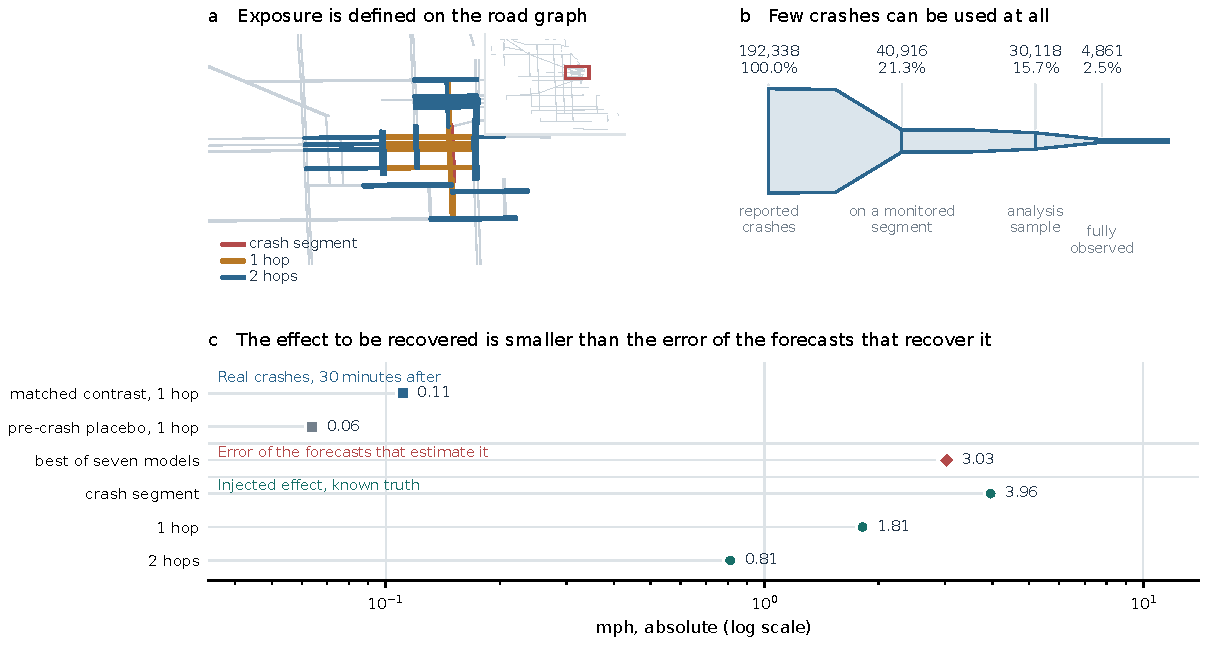
\includegraphics[width=0.97\textwidth]{figure1_study_design.pdf}
\Description{Three panels. A map of the monitored Chicago network with one crash segment, its one-hop ring and its two-hop ring highlighted. A tapering ribbon showing reported crashes surviving each eligibility filter, from 192,338 to 4,861. A dot plot on a logarithmic mph axis placing the injected effect at each ring, the best held-out forecast error, and the matched one-hop association beside its pre-crash placebo.}
\caption{\textbf{What the study can observe.} (a) Exposure rings on the frozen monitored network. (b) Reported crashes surviving each eligibility filter. (c) The same quantities on one absolute scale. The injected effect that estimators must recover is smaller at every ring than the held-out error of the forecasts used to recover it, and the matched one-hop association on real crashes is close to its own pre-crash placebo. Every value is read from the released result bundle.}
\label{fig:overview}
\end{figure*}

\section{Related Work}
\textbf{Estimating traffic incident effects.} Cao et al. compare incident traffic conditions with estimated reference conditions to quantify speed reductions \cite{cao2021traffic}. Li et al. study heterogeneous highway crash effects using doubly robust causal learning \cite{li2024crash}. These approaches emphasize the need for credible comparisons. We examine monitored urban arterial neighborhoods and report matched observational contrasts with sensitivity checks.

\textbf{Graph traffic models.} GCN, GraphSAGE, and DCRNN establish several ways to use road connections for prediction \cite{kipf2017gcn,hamilton2017graphsage,li2018dcrnn}. Their usual evaluation measures forecasting accuracy. We additionally assess whether correct adjacency improves recovery of a known intervention effect. This comparison uses the same model family and evaluation targets under alternative message-passing graphs.

\textbf{Counterfactual learning and interference.} The CASTANET preprint combines spatiotemporal graph learning with incident-effect estimation for traffic forecasting \cite{kitahara2026castanet}. MSCT develops treatment-aware post-crash prediction under time-varying confounding \cite{li2024msct}. Network Deconfounder and network-interference methods formalize treatment-effect estimation when units are connected \cite{guo2020network,ma2021interference,forastiere2022interference}. Exposure mappings also require empirical scrutiny \cite{huber2026exposure}. We focus on an additional model-evaluation question: whether the correct physical adjacency improves known-effect recovery under fixed interventions and targets.

\section{Data and Causal Target}
\subsection{Chicago traffic and the road graph}
We use ten-minute arterial speed observations and geocoded crash reports from the City of Chicago \cite{chicagoSpeeds,chicagoCrashes}. The study covers July 1, 2024 through March 31, 2026. An additional day of crash records identifies incidents preceding the first speed windows. Times are aligned to Chicago local time.

Nodes represent monitored road segments. Their geometry is matched to a fixed OpenStreetMap network. We retain directed connections for GNN message passing. A reported crash is assigned to a monitored segment when its coordinates match a qualifying road edge within 50 meters. This fixed threshold and the limited set of monitored roads affect which crashes enter the analysis.

For exposure, we treat adjacency as undirected. Let $R_0(s)$ contain incident segment $s$, and let $R_1(s)$ and $R_2(s)$ denote the exclusive one- and two-hop neighborhoods. The rings describe connectivity among monitored segments. They do not determine travel direction or imply a specific physical propagation path. Missing speeds are masked separately from recorded zero speeds.

\begin{table}[t]
\centering
\caption{Study coverage and selected event counts. Audit and event-study stages use different eligibility rules.}
\label{tab:data}
\footnotesize
\begin{tabular}{lr}
\toprule
Measurement & Value \\
\midrule
Reported crashes in the study window & 192,338 \\
Assigned to monitored roads & 40,916 \\
Eligible under audit filters & 30,118 \\
Common event-study cohort & 9,275 \\
Mean observed road--time coverage & 56.9\% \\
\bottomrule
\end{tabular}
\end{table}

The source data cover only a subset of road segments and time cells. Table~\ref{tab:data} summarizes coverage and key event counts. Eligibility for the event study also depends on available outcomes, exposure ring, and matched controls. We retain these distinctions when reporting results.

\subsection{Effect definition and identification}
For reported crash $e$ and segment $i$ in exposure ring $k$, let $Y_{eih}(k)$ denote speed at horizon $h$ under exposure to that crash. Let $Y_{eih}(\varnothing)$ denote speed without the index crash. The target removal contrast is
\begin{equation}
\tau_{eih}(k)=Y_{eih}(k)-Y_{eih}(\varnothing),\qquad
h\in\{10,20,\ldots,60\}\ \mathrm{min}.
\label{eq:target}
\end{equation}
A negative value in Equation~\eqref{eq:target} represents a slowdown under the crash. This definition assumes that the exposure mapping adequately describes the relevant intervention and that background conditions can be held comparable.

Matched controls approximate the untreated trajectory only under further assumptions about overlap, consistency, and untreated trends. Common traffic demand may affect both crash risk and speed. Road matching, crash timestamps, and incomplete monitoring introduce additional uncertainty. We therefore interpret real-crash comparisons as \emph{observational contrasts}. The injected interventions provide known outcomes for measuring model recovery error.

\section{Estimation Methods}
\subsection{Matched crash-event contrasts}
Each event uses two hours of pre-crash history and six post-crash ten-minute horizons. The event origin is the last bin before the reported crash. We select up to five control windows from the same incident road and time-of-week slot. Candidate controls must satisfy observation and crash-contamination requirements. Matching ranks candidates by pre-event speed level and trend. We also evaluate controls selected from neighborhood summaries and random candidates.

Let $\overline{Y}_{ei}^{\mathrm{pre}}$ be the observed pre-event mean for target road $i$ in crash event $e$. For matched control period $c$, the road-level difference-in-differences contrast at horizon $h$ is
\begin{equation}
D_{eich} = \left(Y_{eih}-\overline{Y}_{ei}^{\mathrm{pre}}\right)
-\left(Y_{cih}-\overline{Y}_{ci}^{\mathrm{pre}}\right).
\label{eq:did}
\end{equation}
We average controls for each event, road, and horizon. We then average roads within each exclusive exposure ring and assign equal weight to eligible crash events. A crash with more monitored neighbors therefore receives no additional weight solely from its neighborhood size. A fixed-cohort analysis uses events observed across every ring and horizon.

We examine pre-event balance, short pre-event placebos, overlapping crashes, and recorded zero speeds. Each horizon reports its eligible event count. Intervals use event-level standard errors with a nominal 95\% multiplier. They do not correct for dependence between nearby crashes or for the set of horizons tested.

\subsection{Untreated forecasts and residual estimates}
All forecasting models receive twelve ten-minute historical bins and predict the following six bins. We compare persistence and historical-mean predictors with MLP, GCN, GraphSAGE, temporal GRU, and GRU--GCN models. The last model applies temporal recurrent encoding followed by graph convolution. Training uses observed crash-free targets, chronological 70/15/15 splits, an 18-window split embargo, masked MAE loss, and early stopping within 20 epochs.

For crash $e$ on its incident road, let $r_{eh}=Y_{eh}-\widehat Y_{eh}^{(0)}$ be the residual from an untreated-speed forecast. Let $C_{eh}$ be its eligible controls, and let $\mathcal E_h$ be the events observed in both conditions. We compare residuals within matched events:
\begin{equation}
\widehat\tau_h^{\mathrm{res}}=\frac{1}{|\mathcal E_h|}
\sum_{e\in\mathcal E_h}\left(r_{eh}-\frac{1}{|C_{eh}|}
\sum_{c\in C_{eh}}r_{ch}\right).
\label{eq:residual}
\end{equation}
This real-crash residual estimate concerns the incident road. The event-study contrast in Eq.~\eqref{eq:did} covers neighboring rings. For injected interventions, we apply the same residual correction to each eligible event--road--horizon cell. If $\mathcal C_{eih}$ is the set of matched untreated controls, the corrected estimate is
\begin{equation}
\widehat\delta^{\mathrm{corr}}_{eih}
=\left(Y^{\mathrm{sim}}_{eih}-\widehat Y^{(0)}_{eih}\right)
-\frac{1}{|\mathcal C_{eih}|}\sum_{c\in\mathcal C_{eih}}
\left(Y^{(0)}_{cih}-\widehat Y^{(0)}_{cih}\right).
\label{eq:corrected}
\end{equation}
The topology ablation reports MAE of this corrected estimate against the realized injected effect on the eligible cells.

\subsection{Exposure-conditioned outcomes}
We train treatment-aware MLP and GCN models to predict outcomes for four exposure states, $\{\varnothing,0,1,2\}$. Each observed training cell supervises its factual exposure head. An estimated effect is the difference between the exposure-specific and no-crash predictions:
\begin{equation}
\widehat\tau_{ih}^{\mathrm{head}}(k)=
\widehat Y_{ih}(k)-\widehat Y_{ih}(\varnothing).
\label{eq:head}
\end{equation}
The MLP receives neighboring-speed summaries. The GCN uses explicit message passing. The non-graph model is therefore informed about nearby traffic through summaries, while the graph model learns from the adjacency structure. Both methods require adequate support across exposure states to estimate unobserved outcomes.

\section{Experimental Evaluation}
\subsection{Topology comparisons}
We compare three message-passing graphs. \textbf{Real} uses the observed directed road network. \textbf{Self-only} removes messages between distinct roads. \textbf{Relabelled} assigns road connections to incorrect node identities while preserving the graph's edge structure. The underlying exposure rings and injected effects are fixed across these conditions. Degree and betweenness inputs are removed from these ablations to prevent leakage of the original graph.

GCN comparisons use three paired training seeds, 42, 43, and 44. GRU--GCN uses one seed. The relabelled condition uses one fixed permutation. We measure changes in MAE relative to the real-graph model at the same seed and on the same target cells. This design isolates the contribution of the tested adjacency under a fixed model family.

\subsection{Controlled interventions}
We inject known slowdowns into held-out target periods while preserving the historical inputs. The main intervention scales across exclusive rings as $\lambda^k$, with $\lambda=0.45$, and decays over time with a two-bin half-life. Nominal incident-road magnitudes range from 4 to 12 mph. Speeds are bounded below by zero, and evaluation uses the realized intervention after that bound. Each scenario targets up to 200 disjoint events.

\begin{table}[t]
\centering
\caption{Semi-synthetic interventions and the behavior each probes.}
\label{tab:scenarios}
\footnotesize
\begin{tabular}{lp{0.64\columnwidth}}
\toprule
Scenario & Intervention \\
\midrule
B0 & Spatial and temporal decay \\
B1 & Direct-road slowdown with zero neighbor effect \\
B2 & Three-bin slowdown plateau \\
B3 & Placement influenced by pre-event congestion \\
\bottomrule
\end{tabular}
\end{table}

The additive construction has an important consequence. For untreated speed $Y^{(0)}$, true injected effect $\delta$, and predicted untreated speed $\widehat Y^{(0)}$,
\begin{equation}
\left(Y^{(0)}+\delta-\widehat Y^{(0)}\right)-\delta
=Y^{(0)}-\widehat Y^{(0)}.
\label{eq:identity}
\end{equation}
For the raw residual, absolute effect error therefore equals untreated forecast error on the same cells. The matched-control term in Eq.~\eqref{eq:corrected} changes this quantity. We evaluate its error against the known effect and also report the raw residual as a diagnostic. The direct-only scenario assesses false neighboring effects where the true intervention is zero.

\subsection{Outcome metrics and comparability}
Forecast performance is measured by MAE and RMSE on observed held-out cells. Known-effect recovery uses the cell-weighted mean absolute error against realized injections. We compute signed bias by first averaging errors within each event, then averaging events equally. These statistics therefore use different weights. We distinguish comparisons on identical target cells from those using different eligible sets. Model rankings require shared evaluation cells.

\section{Results}
All results below come from a single execution of the frozen experiment matrix. Each reported table is identified by file hash in the released bundle, and the estimators, windows, matching rules, and seeds quoted here were read from the executed stage commands rather than from documentation. One provenance gap remains. The run recorded its code version with a working-tree marker, so the exported results are identified by the bundle and its recorded settings and not by a published commit.

\subsection{Contribution of road topology}
\begin{figure*}[t]
\centering
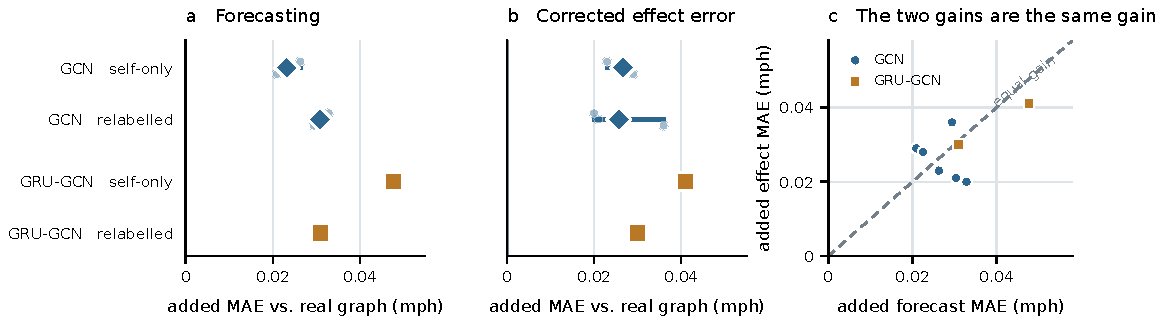
\includegraphics[width=0.96\textwidth]{figure2_topology_results.pdf}
\Description{Three panels. Two horizontal dot plots show how much forecasting and known-effect MAE increase when self-only or relabelled message passing replaces the real network, with zero meaning no difference. A third panel scatters the added effect MAE against the added forecast MAE for the same eight paired contrasts, with the points lying along a dashed line of equality.}
\caption{\textbf{Topology ablation.} (a, b) Added forecast MAE and added matched-corrected B0 effect MAE relative to real adjacency, paired within training seed. Diamonds are GCN seed means, circles individual seeds, squares the single GRU--GCN seed. (c) The same eight contrasts plotted against each other. Points on the dashed line gain exactly as much in effect error as in forecast error.}
\label{fig:topology}
\end{figure*}

The observed adjacency produces the lowest forecasting error and matched-residual B0 error among the tested topology conditions (Figure~\ref{fig:topology}). For the GCN, self-only processing increases forecast MAE by 0.023 mph and corrected effect MAE by 0.027 mph. All three paired seeds have the same direction of difference. These gains are small relative to errors above 3 mph. The corrected effect metric includes forecast residuals and a matched-control adjustment. It is not the raw additive quantity in Eq.~\eqref{eq:identity}.

These two gains are the same gain. Across the eight paired topology contrasts, the mean added forecast MAE is 0.030 mph and the mean added corrected-effect MAE is 0.029 mph, and the contrasts lie along the line of equality (Figure~\ref{fig:topology}c). Equation~\eqref{eq:corrected} accounts for this. The corrected estimate subtracts a matched control residual from the treated residual, so its error is a difference of two forecasting errors and inherits whatever the topology does to forecasting. The experiment therefore does not isolate a benefit of correct adjacency that is specific to counterfactual estimation, which is the question it was built to answer.

Signed bias is the one reported quantity that is not a direct function of forecast accuracy, because a forecaster's systematic error largely cancels between the treated and the control residual. The real graph also ranks first there. Mean absolute pooled bias across three GCN seeds is 0.091 mph with real adjacency, 0.105 mph with self-only processing, and 0.115 mph relabelled. With three training seeds and a single relabelling this ordering is suggestive rather than established, and the GRU--GCN comparison rests on one seed.

\subsection{Matched speed changes after crashes}
\begin{figure*}[t]
\centering
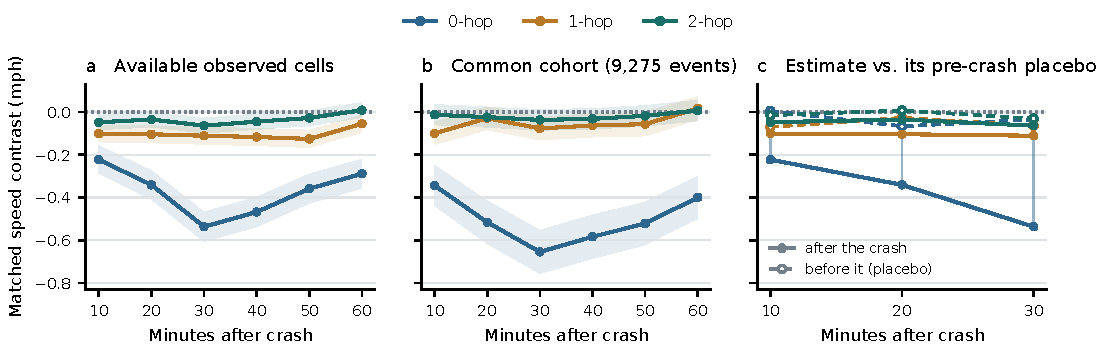
\includegraphics[width=0.96\textwidth]{figure3_observational.pdf}
\Description{Three panels. Crash-associated speed contrasts across 10 to 60 minutes for incident roads and one- and two-hop neighborhoods, first on available observations and then on a fixed cohort of 9,275 events. A third panel places each post-crash estimate beside the same contrast measured before the crash.}
\caption{\textbf{Matched speed contrasts over time.} (a) Available observations. (b) A fixed cohort of 9,275 events observed at every horizon and ring. (c) Each estimate beside its pre-crash placebo, the contrast measured on the same roads before the reported crash time. Shading denotes nominal 95\% event-level intervals.}
\label{fig:observational}
\end{figure*}

Matched differences are largest on crash roads (Figure~\ref{fig:observational}). At 30 minutes, the incident-road contrast is approximately $-0.54$ mph. One- and two-hop contrasts are much smaller. They also depend more strongly on which events have observed neighbor outcomes. Fixing the sample to 9,275 events reduces the neighboring-road magnitudes. The two-hop interval in this cohort includes zero.

\begin{table}[t]
\centering
\caption{Selected one-hop diagnostics at 30 minutes. Matched contrasts are in mph.}
\label{tab:checks}
\footnotesize
\begin{tabular}{lr}
\toprule
Diagnostic & Estimate \\
\midrule
Available observations & $-0.111$ \\
Fixed event cohort & $-0.077$ \\
Exclude overlapping reported crashes & $-0.099$ \\
Exclude recorded zero speeds & $-0.090$ \\
Pre-event placebo & $-0.064$ \\
\midrule
Pre-event level standardized difference & $-0.025$ \\
Pre-event trend standardized difference & $-0.004$ \\
\bottomrule
\end{tabular}
\end{table}

The one-hop matched association is comparable in magnitude to its pre-event placebo (Table~\ref{tab:checks}). It does not provide persuasive evidence of a crash-induced neighboring-road slowdown. Cohort restrictions also reduce its magnitude. Overlap and zero-speed exclusions yield similarly small associations. Six control-drawing rules ran in the reported execution, covering random draws at three seeds, pre-event matching restricted to one and two hops, and matching on the target road. Only the reported rule was collected into the result bundle. \pending{Collect the five remaining matching arms and report the spread of the one-hop estimate across control-drawing rules, with pre-crash trajectories and control-reuse counts.}

\subsection{Forecasting baselines and effect calibration}
\begin{table}[t]
\centering
\caption{Held-out forecasting performance under standard inputs, seed 42. Lower is better.}
\label{tab:forecast}
\footnotesize
\begin{tabular}{lrr}
\toprule
Model & MAE & RMSE \\
\midrule
GRU--GCN & 3.031 & 4.173 \\
GraphSAGE & 3.039 & 4.174 \\
GCN & 3.070 & 4.199 \\
Temporal GRU & 3.073 & 4.219 \\
MLP & 3.105 & 4.242 \\
Historical mean & 3.163 & 4.286 \\
Persistence & 4.139 & 5.629 \\
\bottomrule
\end{tabular}
\end{table}

The standard forecasting comparison is reported in Table~\ref{tab:forecast}. It uses a different input configuration from the topology ablation. For counterfactual evaluation, the B0 benchmark allows the predicted change to be compared directly with the realized injection.

\begin{table}[t]
\centering
\caption{B0 effect errors, seed 42, beside the error of estimating no effect. MAE is averaged over cells. Signed bias is averaged within events and then across events. The residual and exposure-conditioned methods have different eligible cells.}
\label{tab:estimators}
\footnotesize
\begin{tabular}{lrrrr}
\toprule
Estimator & Cells & Cell MAE & At 2 hops & Event bias \\
\midrule
GCN raw residual & 11,948 & 2.984 & 2.981 & $-0.426$ \\
GCN matched residual & 11,948 & 3.202 & 3.171 & $-0.164$ \\
Treatment MLP & 12,053 & 1.208 & 0.641 & $+1.297$ \\
Treatment GCN & 12,053 & 1.210 & 0.656 & $+1.303$ \\
\midrule
Estimate no effect & -- & 1.520$^{\dagger}$ & $\le 2.43$ & $+1.520$ \\
\bottomrule
\end{tabular}

\vspace{2pt}
\footnotesize $^{\dagger}$Event-weighted. Every injected effect is non-positive, so the absolute error of estimating no effect equals the realized magnitude under the same weighting.
\end{table}

\begin{figure}[t]
\centering
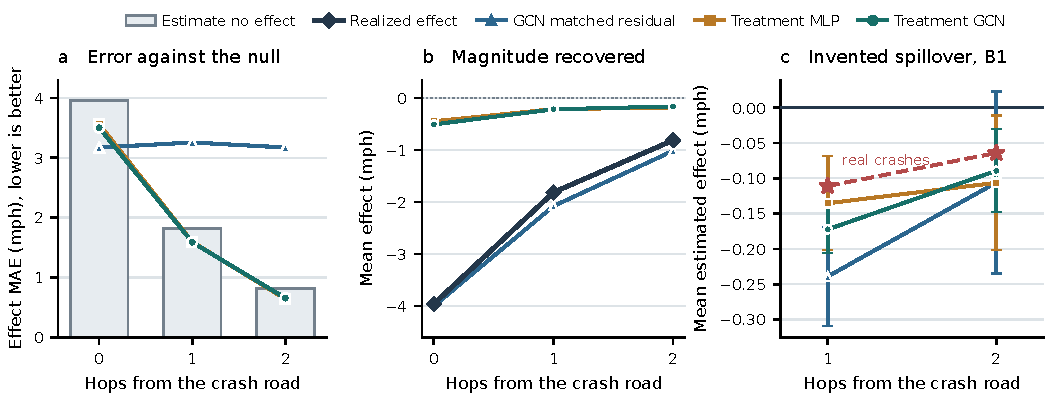
\includegraphics[width=0.99\columnwidth]{figure4_recovery.pdf}
\Description{Two panels on the B0 benchmark. The left panel plots effect MAE by hop for three estimators against bars showing the error of estimating no effect, with the matched-residual estimator above the bars at one and two hops. The right panel plots realized and estimated mean effects by hop, with the exposure-conditioned predictions nearly flat near zero while the realized effect decays from about minus four mph.}
\caption{\textbf{Recovery on B0 against the no-effect null.} (a) Absolute error by ring. Bars are the error of estimating no effect, event-weighted. Lines are cell-weighted MAE. At two hops the ordering holds under any weighting, because the injected effect there cannot exceed 2.43 mph. (b) Realized and estimated mean effects by ring.}
\label{fig:recovery}
\end{figure}

The informative comparison is against estimating no effect at all (Table~\ref{tab:estimators} and Figure~\ref{fig:recovery}a). Both residual estimators are less accurate than that null. At two hops, which carry 6,643 of the 11,948 scored cells, the claim does not depend on weighting. The injected effect there is the event magnitude times $0.45^2$ times a profile bounded by one, so the no-effect estimator cannot exceed 2.43 mph of absolute error, while the residual estimators record 2.98 and 3.17 mph. An error metric on which the best available estimator loses to predicting zero is a weak basis for ranking message-passing topologies, and the topology differences in Figure~\ref{fig:topology}b are 0.03 mph on that metric.

The exposure-conditioned models do improve on the null, by about a fifth pooled, and they do so by shrinking. The treatment GCN estimates approximately $-0.22$ mph against an event-weighted realized slowdown of $-1.52$ mph, which is 14\% of the magnitude, and Figure~\ref{fig:recovery}b shows the attenuation is largest on incident roads. Low absolute error and near-zero predictions are the same behaviour here, because the injected signal is smaller than the forecast noise it sits in. Event-weighted bias and cell-weighted MAE should not be compared using the usual absolute-bias bound.

The residual and exposure-conditioned methods also survive to different cells, 11,948 against 12,053, so their native-support errors are not a paired ranking. Per-cell predictions are now exported, which makes the common-support recomputation possible without retraining. \pending{Recompute cell-weighted bias and MAE on the intersection of the eligible cells, alongside event-weighted summaries.}

\subsection{Null-spillover and intervention stress tests}
All four scenarios in Table~\ref{tab:scenarios} ran in the reported execution, at three seeds each. Benchmark 0 is reported above. The direct-only, plateau, and congestion-placement arms wrote per-arm recovery tables that the result bundle did not collect, so their ring-level errors are not reported here. The direct-only scenario is the one that cannot be inferred from Benchmark 0, because it assigns a true zero to both outer rings and so measures invented spillover directly. Selection on observed pre-crash congestion in the congestion-placement scenario tests sensitivity to an observed selection rule and says nothing about unobserved confounding. \pending{Collect the completed B1 to B3 recovery tables and report false one- and two-hop effects under the direct-only injection.}

\section{Discussion}
The central question was whether correct physical topology helps counterfactual estimation beyond its contribution to forecasting. On the matched-residual metric the answer here is no. The real graph lowers that error, by the same amount that it lowers forecast error, which Equation~\eqref{eq:corrected} predicts for an estimator defined as a difference of two forecasts. Reporting the corrected effect MAE as a second, independent axis of evidence overstates what it adds. Signed bias is the quantity that does carry separate information, and the real graph leads on it, but three seeds and one relabelling cannot establish that ordering.

The deeper issue is the scale of the problem rather than the choice of architecture. The injected effect that B0 asks estimators to recover averages 1.5 mph, and the models forecast untreated speed to about 3 mph. A residual estimator built from those forecasts therefore carries more error than the effect it reports, and at two hops it is less accurate than returning zero. Exposure-conditioned heads escape that bound only by shrinking, which lowers absolute error and loses the magnitude. Neither failure is specific to graph learning, and neither is visible without an explicit null in the table.

Real crashes are associated with lower speeds on monitored incident roads. Neighboring-road contrasts are small and resemble pre-crash placebo differences, so the observational study gives limited support for causal neighboring-road spillovers. Non-significance is not evidence of no effect here. The sample that supports the neighbour estimates is large, and what limits the claim is that an equally large contrast appears before the crash.

The study is limited by incomplete arterial coverage, approximate crash timestamps, a fixed 50-meter road-matching threshold, and undirected hop neighborhoods. Only 2.5\% of reported crashes have every pre-crash and post-crash bin observed on the incident road and a connected road, so the fixed-cohort estimates and the available-case estimates describe different populations. Shared demand and other nearby incidents can affect observed associations. Nominal event-level intervals may understate uncertainty when events share roads or time periods, and we do not report block-clustered intervals. Additive injected shocks leave the forecaster's inputs untouched by construction, which makes them a clean benchmark and an optimistic one. Stronger external evidence requires replicated graph perturbations, the completed null-spillover arms, and clustered observational uncertainty.

\section{Conclusion}
Correct road adjacency gives a small advantage in forecasting, and it gives the same advantage in matched-residual effect error, which is the behaviour of a metric assembled from forecast residuals rather than evidence of a counterfactual-specific gain. Real-crash comparisons show incident-road slowdowns and one-hop associations close to their pre-crash placebos. On known injected effects, residual estimators are less accurate than estimating no effect over most of the scored cells, and exposure-conditioned models beat the null by shrinking their predictions. The useful result is methodological. A counterfactual traffic estimator should be scored against an explicit no-effect null on a stated cell set, and a topology comparison should report the forecasting gain it is built on before claiming anything beyond it.

\noindent\textbf{Reproducibility.} The repository contains the frozen road graph, preprocessing, matching, chronological splits, models, and the submitted experiment matrix. The released bundle carries every reported table with its hash, the resolved input datasets and row counts, and the completed stage list. Each figure is regenerated from that bundle by a single script.

\bibliographystyle{template/ACM-Reference-Format}
\bibliography{references}
\end{document}
